\documentclass{article}
\usepackage{listings}
\usepackage[T1]{fontenc}
\usepackage{titlesec}
\usepackage{graphicx}
\usepackage{amsmath}
\usepackage{xcolor}
\usepackage{amssymb}
\usepackage{circuitikz}
\usepackage{trace}
%\usepackage{minted}
\titleformat{\section}  % which section command to format
  {\fontsize{10}{12}\bfseries} % format for whole line
  {\thesection} % how to show number
  {1em} % space between number and text
  {} % formatting for just the text
  [] % formatting for after the text
  \title{Logika Cyfrowa}
\author{Jakub Gałaszewski} 
\begin{document}
\maketitle
\section{Pokaż, w jaki sposób można wykorzystać pamięci SRAM 4 × 4 (4 słowa po 4 bity) aby skonstruować pamięć 8 × 8 (8 słów po 8 bitów).}
Możemy połączyć każdą jednostkę SRAM w kwadrat 2x2. Wtedy Pierwsza pamięć SRAM będzie odpowiadała za słowa 0-3 i bity 0-3, druga za słowa 0-3 i bity 4-7, trzeci za słowa 4-7 i bity 0-3, a czwarty za słowa 4-7 i bity 4-7. Może to poszerzyć.
\section{W jaki sposób należy podzielić bity adresu pamięci ROM 16-kilobitowej (16384 indywidualnie adresowanych bitów), aby zminimalizować liczbę wejść/wyjść dekodera i multipleksera wchodzących w skład tej pamięci?}
Wiemy że 16384 bitów to $2^{14}$, tak więc aby zminimalizować maksimum wyjść i wejść dekodera oraz multipleksera. Wystarczy policzyć liczbę bitów na pół, czyli dekoder będzie miał 0-6 pierwszych bitów, a multiplekser od 7 do 13, czyli będzie po 7 bitów dla jednego i drugiego.
\section{Ile układów 32K × 8 należy użyć, aby uzyskać pamięć o pojemności 256K bajtów? Ile potrzeba linii adresowych? Ile z tych linii będzie bezpośrednio podłączonych do linii adresowych układów}
Najpierw przeliczmy sobie pojemność w bajtach $256KB = 256K \dot{}8b$, natomiast jeden układ posiada $32K × 8b = 256 Kb$, tak więc potrzeba 8 takich układów. Linii adresowych na układ potrzeba 15, ponieważ $2^{15} = 2^5K = 32K$, czyli sumarycznie potrzebujemy 120 układów ($32*8$) i tyle samo(?) będzie bezpośrednio podłączone do linii adresowych układów.(DOPYTAĆ)
\section{Pokaż, jak zaprogramować układ PLA (odpowiedniego rozmiaru), aby wykonywał operację podnesienia do kwadratu liczby 4-bitowej. Postaraj się, aby użyć jak najmniej zasobów.}
PLA to programowalny układ AND-OR.
TODO
\section{Pokaż, jak wykorzystać makrokomórkę CPLD z wykładu, aby zaimplementować układ, którego wyjściem jest XOR dwóch wejść x, y oraz stanu przerzutnika z poprzedniego cyklu zegara (czyli Dt+1 = Dt xor x xor y). Wyjście przerzutnika może być podłączone do jednego z wejść makrokomórki przez interconnect}
to akurat proste, potem załączyć zdjęcie.
\section{Dla poniższej tabeli stanów narysuj odpowiadający jej diagram stanów. Zminimalizuj automat, narysuj tabelę i diagram stanów zminimalizowanego automatu.}
\begin{center}
	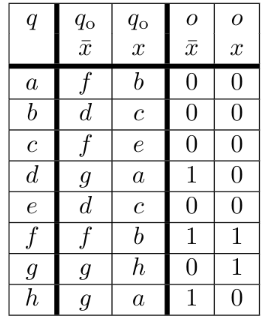
\includegraphics[scale=0.4]{./L10+11Z6.png}
\end{center}
zrobić na kartce i wstawić
\end{document}